\chapter{Construction de clusters de protéines homologues des STIG}\label{chap3b}
\lhead{\emph{Construction de clusters de protéines homologues des STIG}}

   
\section{Récupération des données brutes: les protéines des STIG des génomes}\label{pardonnebrut}
	La collecte des données représente la première étape du pipeline de l'analyse (Figure \ref{figstep1}). Deux sous-ensembles de données brutes peuvent être distingués: i) les séquences génomiques des réplicons et ii) les protéines des STIG.

\begin{figure}[H]
	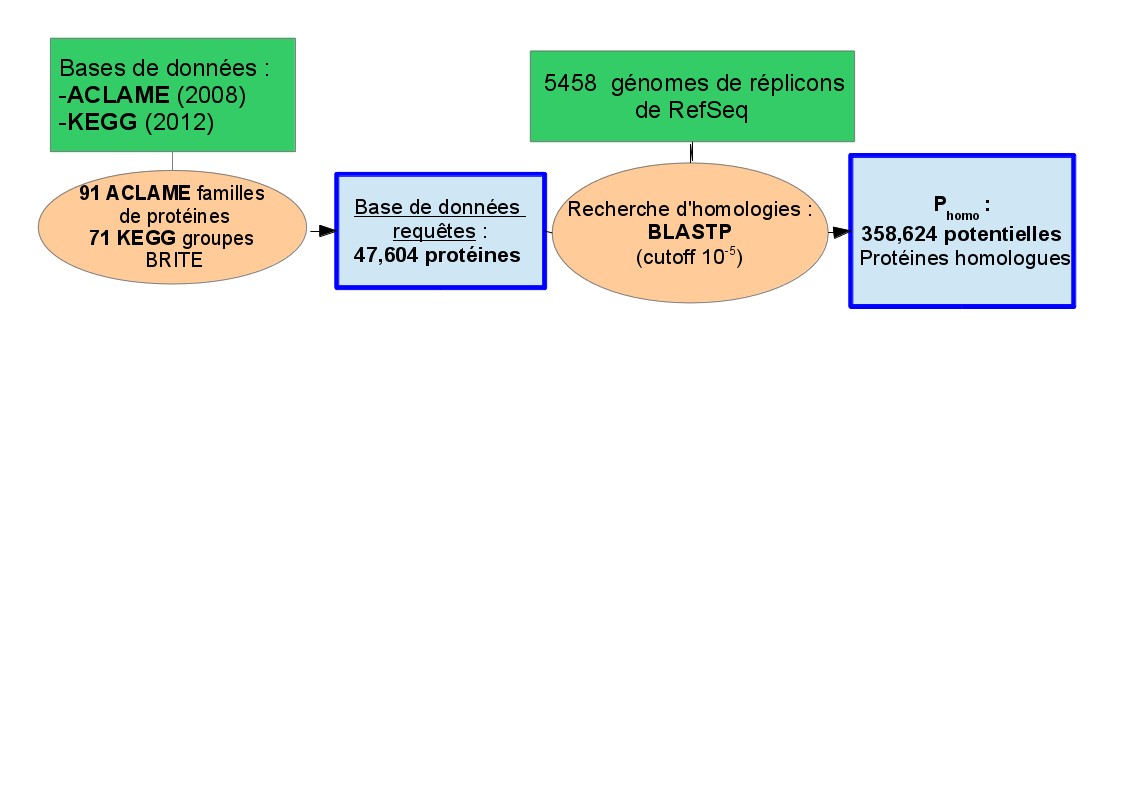
\includegraphics[width=\textwidth, trim= 0cm 12cm 0cm 0cm ,clip]{./img/workflow_sub1.png}
	\caption{Procédure de récupération des données brutes}\label{figstep1}
\end{figure}  

Obtenir une collection quasi-exhaustive des réplicons bactériens séquencés est une tâche aisée car ils sont accessibles dans les bases de données publiques majeures dont celles du NCBI. Par contre, nous avons à faire face à plusieurs difficultés pour la construction d'une base de données des protéines liées aux STIG:
\begin{itemize}
	\item Sélection d'un ou plusieurs système(s) d'annotation protéique parmi ceux proposés par les bases de données existantes.
	\item Sélection des annotations spécifiques aux STIG.
	\item Obtention des données les plus exhaustives possibles pour chaque fonctionnalité des STIG, pour chaque type de réplicon (plasmide et chromosome) et pour toute la diversité taxonomique bactérienne.
\end{itemize}

\subsection{Principales sources publiques de protéines annotées}
    \begin{description}
     \item[NCBI] (National Center for Biotechnology Information) rassemble des données de séquences d'acides nucléiques et de protéines accessibles \textit{via} internet. Les bases de données \textbf{RefSeq} \citep{pruitt2007ncbi} et \textbf{GenBank} \citep{benson2008genbank} sont gérées par le NCBI et constituent des collections de séquences (génomes, gènes, protéines...) parmi les plus importantes disponibles. Les protéines sont annotées partiellement selon leur fonction (vérifiées ou hypothétiques) mais aucun formalisme d'annotation n'est proposé. \textbf{Protein Clusters} regroupe différents clusters de protéines homologues annotées par fonction selon les catégories fonctionnelles des COG (clusters of orthologous groups) \citep{mcentyre2003clusters}, et \textbf{CDD}, rassemble des protéines ou alignements de protéines classés selon leurs motifs structurels \citep{marchler2007cdd}.
      \item[KEGG]  (Kyoto Encyclopedia of Genes and Genomes) est une base de données regroupant des données génomiques, chimiques et systémiques annotées au niveau fonctionnel \citep{Kanehisa2012}. En particulier, les données des génomes complètement séquencés sont hiérarchisées en fonction de leurs propriétés chimiques et systémiques (KEGG BRITE hierarchy), ce qui, concrètement, produit des groupes de protéines regroupées par annotations fonctionnelles.
	\item[ACLAME] (A CLAssification of Mobile genetic Elements) est une base de données dédiée aux données génomiques provenant des \textit{MGE} (Mobile Genetic Element, terme défini par ACLAME) rassemblant des données de phages, plasmides et transposons \citep{leplae2010aclame}. Des clusters de protéines sont accessibles et organisés par familles annotées par des termes de \textbf{G}ene \textbf{O}ntology (GO) \citep{gene2000gene} ou \textbf{PhiGO} (système propre d'ontologie).
	\item[PATRIC]  (PathoSystems Resource Integration Center) est un système d'information libre dont le but est de fournir un support à l'analyse des différents pathogènes bactériens \citep{wattam2014patric}. Elle comprend énormément de génomes bactériens de toutes les espèces, et rassemble les annotations de GO fournies par différentes méthodes d'annotations.
	\item[Pfam] est une large collection de familles de protéines qui sont représentées par des alignements de séquences multiples et des modèles de Markov, et selon leurs domaines fonctionnels \citep{finn2014pfam}.
	\item[TIGRFAM] est une base de données de familles de protéines similaire à Pfam \citep{haft2003tigrfams}.
	\item[PDB] (Protein Data Bank) est une base de données de protéines et séquences nucléotidiques comportant des informations structurales (structures 3D) \citep{rose2013rcsb}.
\end{description}


\subsection{Construction de la base de données requête}\label{donneerequete}
   
	Les bases de données KEGG et ACLAME ont été sélectionnées pour la constitution de la base requête de données protéiques. Leur avantage est de proposer des structures d'annotation plus rigoureuses que celles du NCBI. Les annotations proposées par Pfam et TIGRFAM quant à elles sont principalement liées à la fonction des domaines identifiés sur les protéines et permettent difficilement d'identifier de façon exhaustive des groupes de protéines clairement liées aux STIG.\\
	Le système de hiérarchie BRITE a été utilisé dans la base de données KEGG afin d'identifier \textbf{68} groupes d'orthologues affiliés aux différentes fonctions protéiques d’intérêt (Chapitre \ref{chap1a}). Ce système  permet d'organiser différents objets biologiques (notamment des familles de protéines) fonctionnellement (Figure \ref{figbrite}). Ces 68 groupes d'orthologues (Annexe \ref{AppendiceB}) réunissent un total de \textbf{43.757} protéines.

\begin{figure}[H]
	\hspace{-2cm}
	\begin{minipage}{\textwidth}
		\Tree[.BRITE [.Chromosome [.Prokaryote\_type [.Nucleoid\_associated\_proteins ] [.Partitioning\_proteins ]]] [.DNA\_Replication\_Proteins [.Prokaryote\_type  [.Initiation\_factor Initiation\_factor\_(bactéries) ] [.Termination\_Factors ]]] ]
			\end{minipage}
	\caption[Choix des termes KEGG BRITE]{Choix des termes KEGG BRITE pour la constitution de la base requête de données des protéines liées fonctionnellement aux STIG.}\label{figbrite}
\end{figure}

\textbf{91} familles ACLAME ont été selectionnées selon leurs annotations fonctionnelles (GO et PHI) (Table \ref{aclame}) et regroupent au total \textbf{3.847} protéines (Annexe \ref{AppendiceC}). Le choix des familles ACLAME a été effectué de façon semi-automatique. Différentes familles liées aux STIG ont d'abord été sélectionnées manuellement ce qui a permis d'identifier les annotations pertinentes. Les protéines potentiellement liées aux STIG ont alors été identifiées automatiquement parmi les 18.228 familles de protéines plasmidiques, puis confirmées manuellement.

\begin{table}[H]
\caption[Annotations utilisées pour la selection des Familles ACLAME]{Annotations utilisées pour la selection des Familles ACLAME \citep{leplae2010aclame}.}\label{aclame}
\begin{center}
\begin{tabular}{>{\bfseries\small}l >{\small}l}
{\normalsize Accession}&\textbf{\normalsize Description}\\
\hline
go:0003677 & DNA binding\\
575 & plasmid partitioning protein family ParB/Spo0J\\
go:0015616 & DNA translocase activity\\
576 & plasmid partitioning protein family ParM\\
go:0000146 & microfilament motor activity\\
go:0007059 & chromosome segregation\\
go:0015616 & DNA translocase activity\\
go:0007059 & chromosome segregation\\
go:0016887 & ATPase activity\\
go:0030541 & plasmid partitioning\\
go:0051302 & regulation of cell division\\
phi:0000196 & plasmid copy number control\\
\end{tabular}
\end{center}
\end{table} 
   
      L'ensemble des \textbf{47.604} ($43.757+3.847$) protéines de référence de  KEGG  et ACLAME est noté \textbf{$P_{ref}$}.  L'annotation d'une protéine $p \in P_{ref}$ selon sa famille de référence est désignée par $Ann(p)$. On distingue donc $Ann_{KEGG}(p)$ de $Ann_{ACLAME}(p)$. Les ensembles des familles d'orthologues de KEGG et des familles ACLAME sont notés $Cl_{KEGG}$ et $Cl_{ACLAME}$, respectivement. Enfin, pour tout $C_{i} \in Cl_{KEGG}$ et $C_{j} \in Cl_{ACLAME}$ on désigne par $Ann_{KEGG}(C_{i})$ et $Ann_{ACLAME}(C_{j})$ l'annotation d'une famille KEGG ou ACLAME donnée.
 

\subsection{Récupération des séquences protéiques à partir de RefSeq}
  L'ensemble des séquences complètes de réplicons disponibles a été récupéré le 23/11/2012 \textit{via} le site FTP de RefSeq. Les séquences protéiques (confirmées ou hypothétiques) codées par les gènes de \textbf{5.458} génomes ont été extraites pour un total de \textbf{6.903.452} protéines hypothétiques.
  

\subsection{Sources de biais possibles}\label{parsourcebiais}
	La combinaison des données de KEGG et ACLAME permet de regrouper des protéines annotées d'origines chromosomique et plasmidique. Différentes sources de biais sont possibles:
\begin{itemize}
	\item Certains groupes fonctionnels peuvent être trop spécifiques à un groupe d'espèces. C'est le cas notamment de Hda, DiaA, SeqA, EzrA, SlmA ou RacA qui sont spécifiques de la réplication de \textit{E. coli} et \textit{B. subtilis} notamment, et ne sont pas généralisables à des groupes distants de bactéries.
	\item A l'inverse, certaines familles protéiques (connues ou non) peuvent ne pas être représentées. C'est le cas par exemple de CtrA, Noc ou de YabA. Le choix de ne pas sélectionner ces protéines dépend du fait que celles-ci ne sont pas incluses dans les ensembles de protéines liées aux STIG identifiées précédemment. Ces protéines étant trop spécifiques de certains groupes bactériens, il n'a pas été développé de protocole exclusif d'extraction de leurs séquences. Cela risque de ne pas permettre la discrimination ou l'identification des tendances pour certains groupes de réplicons dont trop peu de leurs STIG seraient représentés dans les protéines sélectionnées.
	\item Il existe un biais d'échantillonnage des familles taxonomiques bactériennes parmi les génomes de réplicons  (Figure \ref{specieplot}). Ce biais peut donner trop de poids aux représentants des familles sur-représentées, et inversement pour les groupes très minoritaires. Il devra en être tenu compte.
	\item Enfin, d'éventuelles erreurs d'annotation des protéines peuvent fausser les résultats. Ce dernier biais, malheureusement, est difficilement estimable dans le cadre de notre étude.
  \end{itemize}
 

\subsection{Recherche d'homologues}\label{paralgoalign}
	Parmi les méthodes permettant d'évaluer l'homologie entre séquences protéiques ou nucléotidiques, on peut distinguer celles qui utilisent un alignement des séquences et celles dites “\textit{alignment-free sequence analysis}” qui répertorient le nombre de mots (ou \textit{k-mers}) communs entre deux séquences.\\
	Le calcul de distances évolutives entre séquences implique classiquement un alignement des séquences, les distances étant estimées à partir des taux de mutation ponctuelle ou des phénomènes d'insertion/délétion observables à partir de l'alignement. Dans certains cas, des phénomènes extrêmes (inversions, recombinaisons multiples) peuvent biaiser les résultats de ces méthodes, qui ne produiront pas d'alignement cohérent malgré l'existence d'homologie entre les séquences.\\
	Parmi les méthodes d'alignement de séquences (Table \ref{align}), on peut séparer celles qui effectuent un alignement global cherchant à aligner tous les résidus des séquences-requête, des méthodes d'alignement local où seulement des parties de séquences peuvent être alignées, ces dernières étant plus intéressantes dans le cas des séquences divergentes. On distingue les méthodes présentant des solutions algorithmiques \textbf{optimales}, des méthodes dites \textbf{heuristiques}, où les résultats sont plus ou moins approchés de l'optimum. On peut de plus distinguer les algorithmes permettant d'aligner des séquences deux à deux, de ceux qui produisent des alignements multiples. Enfin, certains algorithmes requièrent une base de données de séquences à laquelle sont comparées des séquences-requête et produisent des alignements significatifs par rapport à la base de données. 

\newpage
\begin{longtable}{@{\hspace{-2cm}}  >{\bfseries}p{0.18\textwidth} | >{\small}p{0.9\textwidth}}
	\caption[Principaux algorithmes d'alignement de séquences]{Principaux algorithmes d'alignement de séquences de séquences nucléotidiques ou protéiques}\label{align}\\
	 Needleman-Wunsch& (Algorithme de ) \citep{needleman1970general} Algorithme d'alignement global optimal servant à aligner les séquences deux à deux. \\[0.4cm]
	 Smith-Waterman & (Algorithme de ) \citep{smith1981identification} Algorithme d'alignement local optimal servant à aligner les séquences deux à deux. \\[0.4cm]
	BLAST & (\textbf{B}asic \textbf{L}ocal \textbf{A}lignment \textbf{S}earch \textbf{T}ool) \citep{altschul1990basic} Heuristique de recherche et d'alignement local de séquences, à travers une base de données. Différentes phases composent l'algorithme, les principales étant: la recherche de \textbf{\textit{k-mer}}, la construction d'un alignement local à partir des hits et l'évaluation de l'alignement (statistique de  Karlin-Altschul \citep{korf2003blast}). BLAST est une approximation de l'algorithme de Smith et Waterman, et est l'une des méthodes les plus utilisées dans la recherche d'homologie de séquences, le logiciel le plus utilisé étant la suite du NCBI \citep{Camacho2009}. Le programme PSI-BLAST \citep{altschul1997gapped} est une variante de BLAST, qui inclut des procédures itératives de l'algorithme initial afin d'augmenter sa sensibilité à l'identification d'homologues distants.\\[0.4cm]
	HMMER & \citep{finn2011hmmer} Suite de logiciels permettant l'analyse de séquences \textit{via} la création de Modèles de Markov Cachés (HMM pour \textit{Hidden Markov Model}) \citep{eddy1998profile}. À partir d'un alignement multiple de protéines de référence, l'algorithme construit un modèle ou \textit{profile} constitué d'une suite d'états possibles associés à des probabilités de réalisation afin de détecter et d'aligner des séquences homologues potentielles à partir d'une base de données de séquences de référence. \textit{hmmsearch}, algorithme inclus dans la suite HMMER, présente de meilleures performances (sensibilité et spécificité) que BLAST et PSI-BLAST dans la détection d'homologues \citep{Eddy2011}. \textit{Jackmmer}, un autre algorithme de la suite HMMER est une procédure itérative similaire à PSI-BLAST \citep{Eddy2013}.\\[0.4cm]
	 MUSCLE & \citep{edgar2004muscle} Actuellement un des algorithmes les plus performants et les plus populaires d'alignement multiple de séquences. La première étape de l'algorithme compare les séquences deux à deux par une distance de type \textit{k-mer} et produit un arbre de similarité entre les séquences. L'alignement des séquences est ensuite effectué en suivant les branches de cet arbre. Contrairement à BLAST, MUSCLE n'estime pas directement la probabilité qu'un alignement donné soit dû au hasard. 
	 \end{longtable}

	 Bien que produisant des solutions optimales, les algorithmes de Needleman-Wunsch et de Smith-Waterman présentent des complexités trop élevées pour être applicables à l'analyse de près de 7 millions de protéines avec presque 48.000 protéines-requête. Les procédures itératives, bien qu'intéressantes dans la recherche d'homologues éloignés (entre chromosomes et plasmides) présentent deux inconvénients: i) elles convergent moins rapidement, et ii) dans le cas de familles multigéniques (par exemple, les recombinases/intégrases), le feront difficilement et identifieront l'ensemble des protéines codées par la famille multigénique pour une protéine-requête proche de cette famille \citep{Guglielmini2013}. Les méthodes de type HMMER, bien qu'offrant de meilleures performances, dépendent grandement de la qualité des alignements de séquences fournis en entrée. La construction des alignements pour les différents groupes de protéines homologues identifiées constituerait une source supplémentaire de biais. Certains jeux de protéines (les protéines Xer notamment) produisent difficilement des alignements significatifs et une analyse de type HMMER reposant sur un alignement non-significatif constitueront un \textit{profile} source d'erreur \citep{wistrand2005improved}.\\
	\textbf{Le logiciel \textit{blastp} de la suite BLAST+ \citep{Camacho2009} a été choisi pour sa rapidité et sa fréquente utilisation dans la communauté pour le calcul de similarité de protéines.} Le seuil de rejet est fixé pour une $\mathbf{e_{value}}$ (probabilité d'obtenir un alignement significatif par hasard sachant la base de données et la protéine de référence) inférieure à $10^{-5}$. Les scores de BLAST sont calculés par rapport au nombre $r$ d'alignements locaux détectés (hits) de façon heuristique lors de la recherche de \textit{k-mers} \citep{korf2003blast}. Le calcul de la $e_{value}$ par BLAST peut être résumé par:
	\begin{equation}
		\begin{split}
			e_{value}&=-ln(1-p_{value})\\
			&\textrm{où:}\\
			p_{value}&=\frac{p_{value}'}{\beta^{r-1}(1-\beta)}\\
			&\textrm{avec:}\\
			p_{value}'&=\frac{e^{-S_{sum}}S_{sum}^{r-1}}{r!(r-1)!}  
		\end{split}
	\end{equation}
et où $\beta$ est une constante fixée. $S_{sum}$ est une fonction de la somme des scores $S_{i}$ des hits détectés significatifs et de différentes variables telles que la taille $T$ de l'espace de recherche selon l'algorithme utilisé \citep{korf2003blast}:
	\begin{equation}
		S_{sum}=K\sum_{i=1}^{r}S_{i}+f(r,T)
	\end{equation}
avec $K$ constante. Les $S_{i}$, scores des hits d'un alignement de deux séquences $s^{S_{i}}_{1}$ et $s^{S_{i}}_{2}$ de longueur $n$ peuvent être estimés par une équation de la forme  \citep{korf2003blast}:
	\begin{equation}
		S_{i}=\sum_{j=1}^{n} ln\left(\frac{Q_{s^{S_{i}}_{1},s^{S_{i}}_{2}}[j]}{P(s^{S_{i}}_{1}[j]).P(s^{S_{i}}_{2}[j])}\right)
	\end{equation}
où $P(s^{S_{i}}_{1}[j])$ et $P(s^{S_{i}}_{2}[j])$ sont les fréquences d’occurrences du $j$-ème caractère dans l'espace de recherche de  $s^{S_{i}}_{1}$ et de $s^{S_{i}}_{2}$ respectivement et  $Q_{s^{S_{i}}_{1},s^{S_{i}}_{2}}[j]$, la fréquence d'occurrences de la paire formée par le $j$-ème caractère de $s^{S_{i}}_{1}$ et de $s^{S_{i}}_{2}$ dans l'espace de recherche. \\
\\
	Certains travaux ont étudié le lien entre score et pertinence biologique des différents algorithmes de recherche de similarité de séquence \citep{Eddy2011}. En particulier, il a été mesuré qu'une $e_{value}$ inférieure à $10^{-3}$ entre deux protéines correspond à 99\% à des homologues fonctionnels (selon Pfam et leurs annotations de clan et pour une base de données de taille 192.987) \citep{Boekhorst2007}. Un \textbf{\textit{cutoff}} à $10^{-5}$ a été choisi et semble garantir un maximum de pertinence dans la recherche d'homologies fonctionnelles entre les protéines-requête et les protéines identifiées. Un des biais peut cependant provenir de protéines contenant des domaines fonctionnels multiples et pouvant présenter des $e_{value}$ très faibles avec des protéines partageant un de leurs domaines quoique possédant des fonctions totalement différentes \citep{Song2007}.\\ 
	\\
L'analyse des \textbf{6.903.452} protéines par les \textbf{47.604} protéines reliées aux STIG par \textit{blastp} en utilisant une $e_{value}$ seuil de $10^{-5}$ et les paramètres par défaut (\citep{Camacho2009} a identifié \textbf{358.624 protéines homologues}, dont l'ensemble est désigné \textbf{$P_{homo}$}. La $e_{value}$ d'une protéine $p$ par rapport à une protéine $q$ sera notée: $e_{value}(p,q)$.



\section{Réalisation de clusters d'homologues protéiques et fonctionnels}\label{parclusterhomo}
	Les protéines liées fonctionnellement aux STIG récupérées sont ensuite utilisées comme référence pour identifier des homologues fonctionnels dans les 5.125 réplicons de notre jeu de données. Ensuite, les protéines identifiées sont partitionnées selon leurs homologies de séquences \textit{via} une analyse de clustering \textbf{afin de créer des unités d'homologies structurales et fonctionnelles}. Enfin, une procédure de “nettoyage” est effectuée afin d'exclure les clusters les plus biaisés (Figure \ref{figstep2}). 
  
\begin{figure}[H]
	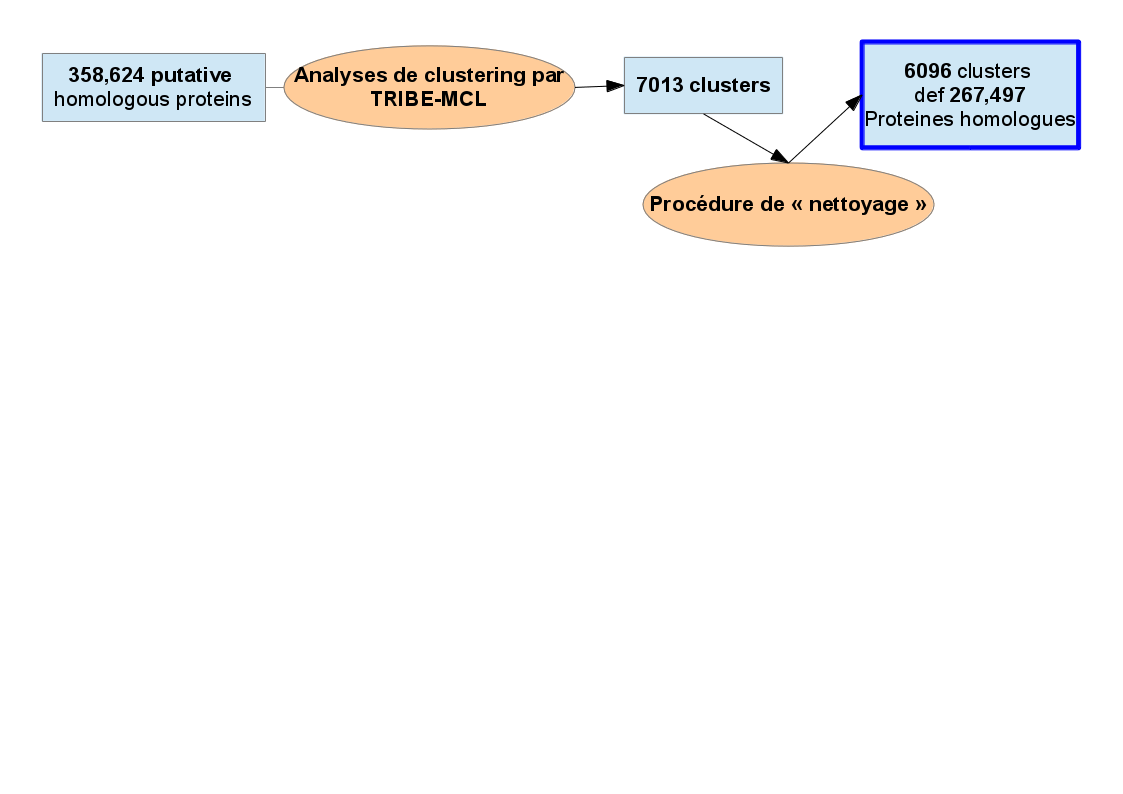
\includegraphics[width=\textwidth, trim= 0cm 14cm 0cm 0cm ,clip]{./img/workflow_sub2.png}
	\caption{Procédure de clustering des protéines}\label{figstep2}
\end{figure}  
	
Le choix et le paramétrage d'un algorithme de calcul d'homologie de séquences est suivi du choix et du paramétrage d'un algorithme de clustering de séquences protéiques. Différentes méthodes d'évaluation des clusters sont introduites. 



\subsection{Clustering des protéines}
\subsubsection{Définition}
	La majorité des algorithmes de clustering de séquences protéiques (ou nucléotidiques) reposent sur le calcul préalable d'une matrice de comparaison (aussi appelée matrice de distance ou de dissimilarité) de séquences deux à deux:
	\begin{description}
		\item[$\bullet$]  Pour un ensemble de $n$ protéines $P=\{p_{1},...,p_{n}\}$ et une distance $d$ calculant un degré de dissimilarité de séquence $d(p_{i},p_{j})$ entre deux protéines $p_{i}$ et $p_{j}$, soit $M^{d}$ la matrice de distance où: 
			\begin{equation}
				M_{ij}^{d}=d(p_{i},p_{j})
			\end{equation}
		\item[$\bullet$] $S^{d}$, la matrice de similarité, est alors définie par :
			\begin{equation}
				S^{d}_{ij}=1-\frac{d(p_{i},p_{j})}{d_{max}}
			\end{equation}
		\item[$\bullet$] Les graphes d'\textbf{I}nteraction \textbf{P}rotéines-\textbf{P}rotéines (\textbf{IPP}) sont des graphes où $S^{d}$ est la matrice d'adjacence du graphe $G=(P,E,S^{d})$, où $E$ est l'ensemble des couples $(p_{i},p_{j})$ pour lesquels une homologie significative a été detectée.
	\end{description}



\subsubsection{Principe}    
     Les algorithmes de calcul de similarité de séquences (Table \ref{align}) sont généralement utilisés pour le calcul de $e_{value}$ qui servent de distances inter-protéiques. La majorité des méthodes de clustering de protéines sont en fait des algorithmes de détection de communautés appliqués aux IPP \citep{Brohee2006,li2010computational}. Il existe de plus des critères externes spécifiquement développés pour les IPP. Un des biais potentiels dans l'utilisation des $e_{value}$ des algorithmes en tant que distances est qu'elles ne sont pas obligatoirement \textbf{métriques}. En effet, \textit{blastp} et \textit{phmmer}, par exemple, produisent des $e_{value}$ telles que $d(p_{i},p_{j}) \neq d(p_{j},p_{i})$\\
 
 
\subsubsection{TRIBE-MCL}
	L'algorithme de clustering \textbf{TRIBE-MCL} \citep{Enright2002} a été choisi pour son efficacité, démontrée notamment dans la construction des familles ACLAME \citep{leplae2010aclame}, pour sa capacité à regrouper des protéines multi-domaines \citep{Enright2002,Frech2010} et pour ses meilleures performances dans l'identification de familles protéiques \citep{Frech2010,apeltsin2011improving}. \\
	TRIBE-MCL est dérivé de l'algorithme Markov Cluster (MCL) \citep{van2000graph} qui est une méthode de détection de communautés. Le principe de l'algorithme est de capturer des clusters de protéines, régions du graphe où les protéines sont relativement plus interconnectées, en simulant des trajets aléatoires dans le graphe selon l'hypothèse qu'un trajet aléatoire dans un cluster tendra davantage à rester dans ce cluster que d'en sortir. Ces trajets aléatoires sont simulés \textit{via} des opérations sur la matrice d'adjacence du graphe par deux opérations matricielles: \textit{expansion} et \textit{inflation} \citep{Enright2002}. L'expansion a pour effet de dissiper les trajets aléatoires au sein des clusters, et l'inflation élimine les trajets inter-clusters. L'opération d'inflation est sous le contrôle d'un opérateur $gr$ qui, pour des valeurs élevées, augmente le “resserrement” (ou \textbf{granularité}) des clusters obtenus. Une valeur de $gr$ supérieure à 1 permet théoriquement la création de clusters. \\
TRIBE-MCL prend comme mesure de similarité entre deux protéines $p_{i}$ et $p_{j}$ :
	\begin{equation}
		d(p_{i},p_{j})=-log_{10}(e_{value}({p_{i},p_{j})})
	\end{equation}
	L'efficacité de TRIBE-MCL à reconstruire des familles protéiques dépend grandement de la granularité choisie et sera influencée par la nature des familles de protéines étudiées \citep{Frech2010,apeltsin2011improving}.  Ainsi, \textbf{la valeur optimale de $gr$ dépend du jeu de protéines analysé et de la question qu'on se pose.} 


\subsection{Identification des domaines fonctionnels des protéines}\label{pardomaine}
	Afin d'évaluer les clusters formés, les protéines ont été caractérisées selon leurs domaines fonctionnels. Pour l'identification des domaines des 358.624 homologues et des 47.604 protéines de référence, le programme \textit{hmmscan} de la suite HMMER a été utilisé avec la base de données Pfam du 03/03/2013 comme base de données de référence, et, comme valeurs seuils, $e_{value}<10^{-5}$ et  $ce_{value}<10^{-5}$ (\textit{conditionnal $ce_{value}$}). La $e_{value}$ pour un domaine est similaire à la $e_{value}$ précédemment définie. La $ce_{value}$ d'un domaine désigne la probabilité que le domaine ne soit pas significatif sachant que la protéine sur laquelle est trouvé le domaine est un vrai homologue d'une protéine de la base de données requête \citep{finn2011hmmer}. Les valeurs des autres paramètres sont celles par défaut \citep{Eddy2013}. L'ensemble des domaines identifiés dans un ensemble de protéines $P$ est noté $D_{P}$. De même, l'ensemble des domaines identifiés dans une protéine $p$ est noté $D_{\{p\}}$.  \textbf{1.175.018} et \textbf{127.853} profiles ont ainsi été identifiés sur les 358.624 protéines de $P_{homo}$ (ensemble des protéines homologues) et les 47.604 protéines de $P_{ref}$ (ensemble des protéines de référence), respectivement. \textbf{1711} profiles différents sont identifiés (Figure \ref{figdomain}), montrant l'hétérogénéité des protéines présentes.
	
\begin{figure}
	\begin{center}
	\begin{subfigure}{0.8\linewidth}
		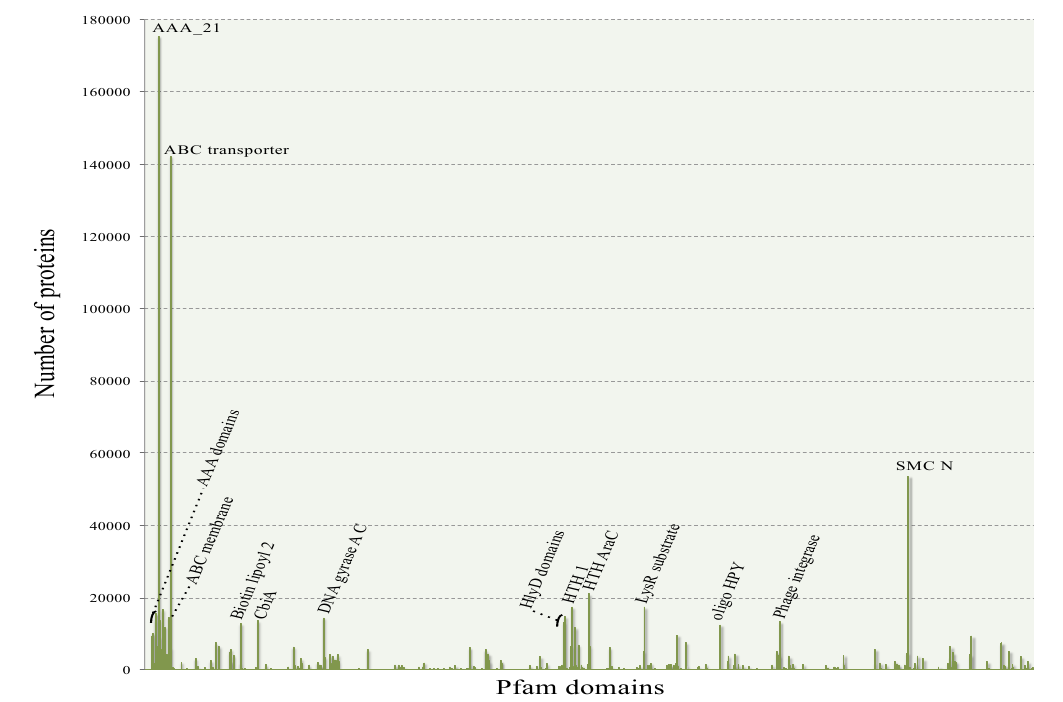
\includegraphics[width=\textwidth]{./img/domain_occurence.png}
		\caption{Distribution des domaines Pfam}\label{figdomain1}
	\end{subfigure}
	\\
	\begin{subfigure}{0.8\linewidth}
		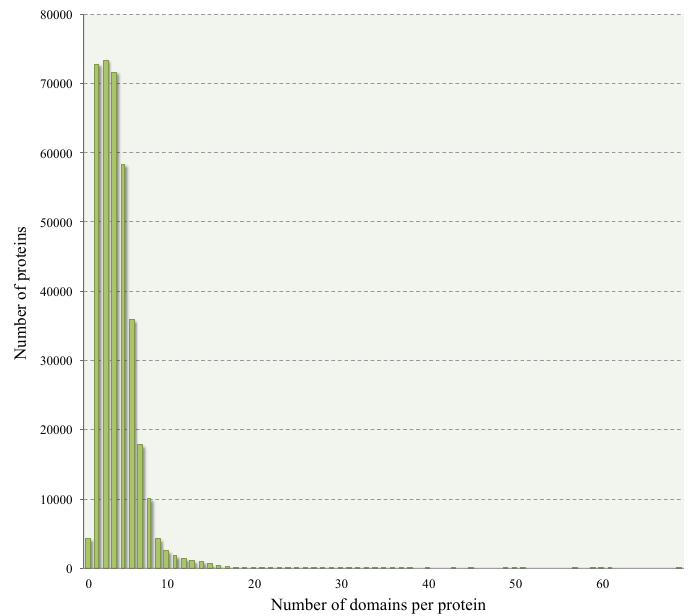
\includegraphics[width=\textwidth]{./img/domain_per_prot.png}
		\caption{Nombre de domaines par protéine}\label{figdomain2}
	\end{subfigure}
	\caption[Distribution des types et nombres d'occurence des profiles dans $P_{homo}$]{Distribution des types et nombres d'occurence des profiles dans $P_{homo}$. \ref{figdomain1}: Histogramme de l’occurrence des 1711 domaines Pfam identifiés. \ref{figdomain2}: Distribution des nombres de domaines Pfam par protéine.}
	\label{figdomain}
	\end{center}
\end{figure}



\subsection{Critères d'évaluation des clusters}
      L'évaluation des IPP se fait généralement sur des critères externes en les comparant à des familles ou classes de protéines de référence \citep{nepusz2012detecting}. 
\begin{description}
\item[$\blacktriangleright$] Il est possible d'utiliser des indices dérivés de la sensibilité/spécificité et du $F_{score}$ (éq. \ref{eqsensitive}) \citep{Brohee2006}.
\item[$\blacktriangleright$] D'autres chercheurs proposent d'évaluer la $p_{value}$ d'un cluster par rapport à une classe de référence selon leurs tailles \citep{li2010computational}. Pour un cluster $C$ contenant $k$ protéines appartenant à une classe de référence $F$, la probabilité que ce cluster ne soit pas formé par hasard selon $F$ est égale à:
      \begin{equation}\label{pvalue}
        p_{value}=1-\sum_{i=1}^{i=k-1}{\frac{ {|F| \choose i}{|P|-|F| \choose |C|-i} } {{|P| \choose |C|}}} 
      \end{equation}
\item[$\blacktriangleright$] Un autre indice important dans la selection de la granularité pour les IPP est l'\textit{intra-cluster clustering coefficient} (ICCC) \citep{Lima-Mendez2008,VanHoudt2012}. Soit une protéine $p$ de $P$, appartenant à un cluster $C$, et ayant un ensemble $N$ de protéines voisines incluses dans $C$, pour tout $i,j$ tels que $p_{i},p_{j} \in N$, le \textit{clustering coefficient} $CC_{p}$ de $p$ est défini par:
      \begin{equation}\label{ccv}
      	CC_{p}=\frac{\sum_{i=1}^{|N|-1}\sum_{j=i+1}^{|N|}S^{d}_{i,j} }{|N|.(|N|-1)/2}
      \end{equation}
L'ICCC est alors défini par : 
      \begin{equation}
      	ICCC = \sum_{p \in P}CC_{p}
      \end{equation}
\item[$\blacktriangleright$] Différents indices ont été utilisés pour répondre aux deux objectifs suivants: i) obtenir des clusters suffisamment homogènes en homologues fonctionnels et, ii) analyser les similitudes/dissimilitudes des réplicons \textit{via} les clusters obtenus. Deux types de références sont identifiables dans les jeux de données: i) les familles de protéines ACLAME et KEGG et leur annotations, et ii) les domaines Pfam identifiés.\\
 Pour tout $p \in P_{homo}$ et tout $p' \in P_{ref}$, une première annotation de $p$ est donnée par:
      \begin{equation}\label{eqannot}
      Ann(p)=Ann(p') \iff e_{value}(p,p')=min\{e_{value}(p,p'')| \: p'' \in P_{ref}\}
      \end{equation}
\begin{description}
 \item[\textbullet] L'objectif est d'estimer l'homogénéité en terme d'annotation des différents clusters mais l'\textbf{\textit{exhaustivité}} des clusters n'est pas recherchée. Pour cela un indice externe de comparaison dérivé du Biological Homogeneity Index (BHI) \citep{Datta2006} est alors calculé. Soit un clustering $Cl$ composé de $k$ clusters: $Cl=\{C_{1},...,C_{k}\}$. Le BHI est alors défini par:
	\begin{equation}
      	BHI=\frac{1}{|Cl|}\sum_{i=1}^{|Cl|}c_{i}
      \end{equation}
où $c_{i}$ est défini par:
      \begin{equation}\label{bhiwci}
      	c_{i}=\frac{2}{|C_{i}|.(|C_{i}|-1)}\sum_{p,q \in C_{i}}d(p,q)
      \end{equation}
sous l'hypothèse que, pour tout $p \in C_{i}, \; \exists \; Ann(p)$ où $d(p,q)$ est défini par:
      $$d(p,q) = 
      \begin{cases}
       1 & \text{si } Ann(p)=Ann(q)\\
       0 & \text{sinon }
      \end{cases}
      $$
Contrairement à l'indice initial, la constante “$2$” est ajoutée pour que le dénominateur soit de la forme $\frac{N.(N-1)}{2}$, qui est le nombre de paires dans $N$ éléments (on compare le nombre de \textit{cas} observés sur le nombre de \textit{cas} possibles, ainsi l'éq. \ref{bhiwci}, tout comme l'éq. \ref{ccmci} ci-après, est de la forme de l'éq. \ref{ccv}). En d'autres termes, le BHI est une mesure simple à interpréter, prenant ses valeurs dans $[0,1]$, qui est maximum si, pour tout cluster $C_{i}$ de $Cl$, toutes protéines $p$ de $C_{i}$ possèdent une même annotation: $Ann(p)$. Le BHI ne prend cependant pas en compte les potentielles grandes différences de taille entre clusters (ce qui est notre cas: Figure \ref{figclustersize}). Une correction du BHI est alors apportée pour donner le \textit{weighted BHI} (BHIw): 
	\begin{equation}\label{bhiw}
		BHIw=\frac{1}{|P|}\sum_{i=1}^{|Cl|}c_{i}.|C_{i}|
	\end{equation}
où $|P|$ est le nombre total de protéines du clustering (dans notre cas $|P_{homo}|$). 

\item[\textbullet] Avec pour objectif de mesurer l'\textit{\textbf{homogénéité}} des clusters, c'est-à-dire leur capacité à contenir des protéines ayant des domaines fonctionnels similaires, l'indice \textit{Conservation Consistency Measure} (CCM) est introduit. Le CCM est défini par:
	\begin{equation}\label{ccm}
		CCM =\frac{1}{|P|}\sum_{i=1}^{|Cl|}c'_{i}.|C_{i}|
	\end{equation}
où $c'_{i}$ est défini par:
	\begin{equation}\label{ccmci}
		c'_{i}=\frac{2}{|C_{i}|.(|C_{i}|-1)}\sum_{p,q \in C_{i}}d_{Jaccard}(D_{\{p\}},D_{\{q\}})
	\end{equation}
et où $d_{Jaccard}$ est la distance de Jaccard pour deux ensembles. L'indice CCM prend ses valeurs dans $[0,1]$. Une valeur proche de 0 indique des clusters qui contiennent des protéines ayant des domaines similaires.\\

\item[\textbullet] Enfin, on peut aussi calculer la proportion d'annotation majoritaire pour chaque cluster. Soient un cluster $C$, $Ann_{max}^{C}$ l'annotation majoritaire des protéines de $C$, et $N_{Ann_{max}^{C}}$ le nombre de fois que $Ann(p)=Ann_{max}^{C}$ pour tout $p \in C$. On définit $Pr_{ Ann_{max}}$ par:
	\begin{equation}\label{eqpourc}
		Pr_{ Ann_{max}}=\frac{N_{Ann_{max}^{C}}}{|C|}
	\end{equation}
\end{description}
\end{description}


      
\subsection{Génération de clusters aléatoires}\label{parclustaleat}
	L'évaluation des clusters formés ainsi que les procédures de “cleaning” (ci-après) font intervenir des clusters de protéines engendrés aléatoirement. Une protéine étant uniquement caractérisée par le nombre et le type de domaines qu'elle comporte, on peut distinguer trois processus aléatoires indépendants intervenant dans la génération aléatoire d'un cluster de protéines:
\begin{description}
	\item[$\bullet$] le nombre de protéines du cluster,
	\item[$\bullet$] le nombre de domaines fonctionnels présents dans une protéine donnée,
	\item[$\bullet$] le type d'un domaine donné.
\end{description}

\subsubsection{Variables}
Soit $X_{k}$, $X_{d}$ et $X_{t}$ les variables aléatoires discrètes et indépendantes correspondant aux nombre de protéines par cluster, nombre de domaines et type d'un domaine, respectivement. Les ensembles des valeurs possibles $E_{k}$, $E_{d}$ et $E_{t}$ sont alors déduits des données:
	\begin{description}
		\item[$\mathbf{E_{k}}$] prend ses valeurs entre $1$ (le nombre minimum de protéines dans un cluster) et $max\{|C|\;|\; C \in Cl\}$ pour un $Cl$ donné.
		\item[$\mathbf{E_{d}}$] prend ses valeurs entre $0$ (le nombre minimum de domaines fonctionnels identifiés dans une protéine donnée) et $max\{|D_{\{p\}}|\; p \in P_{homo}\}$.
		\item[$\mathbf{E_{t}}$] prend ses valeurs dans $D_{P_{homo}}$.
	\end{description}	    
De même, l'estimation des lois de probabilités de $P_{X_{k}}$, $P_{X_{d}}$ et $P_{X_{t}}$ se fait à partir des données:
	\begin{description}
		\item[$\mathbf{P_{X_{k}}}$] Soient $O_{Cl}=\{|C_{i}|, \;  C_{i} \in Cl\}$ la distribution des tailles des clusters d'un clustering, $Q^{q}_{O_{Cl}}=\{Q_{1},..,Q_{q}\}$ les q-quantiles de $O_{Cl}$, et $x_{(p/q)}$ la première valeur de $Q_{p}$ (avec $x_{((q+1)/q)}=+\infty$). On estime alors que:
			\begin{equation}\label{Xk}
				P_{X_{k}} \to
				\begin{dcases}
				P(x_{p/q}\leq X_{k}<x_{(p+1)/q})= \frac{|Q_{p}|}{|O_{Cl}|} & \textrm{ où } p \in \{1,...,q\}\\
				P(X_{k}=x_{p_{i}})=U([x_{p/q},x_{(p+1)/q}[)) &  \textrm{ où }  x_{p_{i}} \in [x_{p/q},x_{(p+1)/q}[\\
				\end{dcases}
			\end{equation}
		où $U$ est la loi uniforme discrète. D'une part la probabilité d'obtenir une valeur de taille $k$ incluse dans un certain intervalle dépend du nombre d'observations présentes dans cet intervalle et, d'autre part, toutes les valeurs de $k$ au sein d'un intervalle donné ont la même probabilité d'être tirées.
		\item[$\mathbf{P_{X_{d}}}$] En suivant la même démarche que pour $P_{X_{k}}$, on estime  que:
     			\begin{equation}\label{Xd}
				P_{X_{d}} \to
				\begin{dcases}
				P(x_{p/q} \leq X_{d}<x_{(p+1)/q})= \frac{|Q_{p}|}{|O_{P_{homo}}|} & \textrm{ où }   p \in \{1,...,q\}\\
				P(X_{k}=x_{p_{i}})=U([x_{p/q},x_{(p+1)/q}[)) &  \textrm{ où }  x_{p_{i}} \in [x_{p/q},x_{(p+1)/q}[\\      
				\end{dcases}
			\end{equation}
		avec  $O_{P_{homo}}$ la distribution du nombre de domaines par protéine des protéines de $P_{homo}$ et avec $Q_{p} \in Q^{q}_{O_{P_{homo}}}$.
		\item[$\mathbf{P_{X_{t}}}$] Soit $d$ un domaine de $D$. On note $N_{d}^{D}$ le nombre d'occurrences de $d$ dans $D$. $P_{X_{t}}$ est alors simplement estimé par: 
			\begin{equation}\label{Xt}
				P(X_{t}=d)=\frac{N_{d}^{D_{P_{homo}}}}{|D|}
			\end{equation}     
     \end{description}
La création d'un cluster aléatoire s'effectue par un premier tirage avec remise sur $X_{d}$ donnant la taille $x_{k}$ du cluster. On effectue alors $x_{k}$ tirages avec remise sur $X_{d}$ et, pour chaque valeur $x_{d}$ obtenue, on effectue finalement $x_{d}$ tirages avec remise sur $X_{t}$.   
    
\subsubsection{Loi de probabilité des clusters aléatoires}
	Les variables aléatoires $X_{k}$, $X_{d}$ et $X_{t}$ étant indépendantes, soient $X_{C}$ et $X_{Cl}$ les variables indépendantes discrètes correspondant aux tirages d'un cluster aléatoire et d'un clustering aléatoire, respectivement. Soient $C_{k,P}$, un cluster aléatoire constitué d'un ensemble de $k$ protéines $P=\{p_{1},...,p_{k}\}$, et $Cl_{rand}=\{C_{k_{1},P_{1}},...,C_{k_{z},P_{z}} \}$, un clustering aléatoire de $z$ clusters. On peut alors estimer que:
	\begin{equation}
		P(X_{C}=C_{k,P})=P(X_{k}=k).\prod_{p_{i} \in P}P(X_{d}=|D_{p_{i}}|).\prod_{d_{j} \in D_{p_{i}}}P(X_{t}=d_{j})
	\end{equation}
et que:
	\begin{equation}
		P(X_{Cl}=Cl_{rand})=\prod_{C_{k_{i},P_{i}} \in Cl_{rand}}P(X_{C}=C_{k_{i},P_{i}})
	\end{equation}

\subsubsection{Vérification par test d'hypothèses}
    Lorsqu'est calculé un clustering aléatoire $Cl_{rand}$ par rapport à un clustering observé $Cl$, une procédure de vérification est effectuée afin d'estimer si $O_{Cl_{rand}}$ et $O_{Cl}$, les distributions de taille des clusters de $Cl_{rand}$ et $Cl$, respectivement, suivent la même loi. Pour cela, un test d'indépendance du $\chi^{2}$ est réalisé entre $Q_{O_{Cl_{rand}}}^{p}$ et $Q_{O_{Cl}}^{p}$. Pour une $p_{value}$ du test supérieure à 0.05, on estime que les deux distributions ne sont pas statistiquement différentes.


\subsection{Protocole analytique}
    Pour chaque protéine de $P_{homo}$, une analyse \textit{blastp} est conduite sur $P_{homo}$ avec une valeur seuil de $e_{value}$ de $10^{-5}$ permettant l'obtention d'une matrice de similarité $S^{d}$, avec $d$ les $e_{value}$ données par \textit{blastp}. L'algorithme TRIBE-MCL est ensuite lancé sur $S^{d}$ en utilisant les granularités $gr$ suivantes: $(2,3,4,5,6,7,8)$, et les indices CCM, BHI et BHIw sont alors calculés pour les différents $gr$. La variance des scores des trois indices obtenus avec des clustering aléatoires (non représentée) est globalement très faible (de l'ordre de $10^{-5}$). La génération des clusters aléatoires a été réalisée en utilisant 1000 et 20 q-quantiles pour $O_{Cl}$ et $O_{D_{P_{homo}}}$, respectivement, avec $Cl$, les clusterings obtenus pour les différents $gr$. L'adéquation des distributions $O_{Cl}$ et $O_{Cl_{rand}}$ par le test du $\chi^{2}$ est estimée en utilisant 100 q-quantiles.
  
    
\subsubsection{Choix d'un $gr$ de travail}
	Les différents indices confirment l'efficacité de TRIBE-MCL pour la création de partitions pertinentes dans le cas de protéines homogènes en annotations et en contenu de domaines fonctionnels (Figure \ref{figclusteval}). 
	
\begin{figure}[H]
	\begin{center}
	\begin{tabular}{@{\hspace{-1.5cm}}cccc}
	\begin{turn}{90}\scriptsize\hspace{1.5cm} score BHI et BHIw \end{turn}&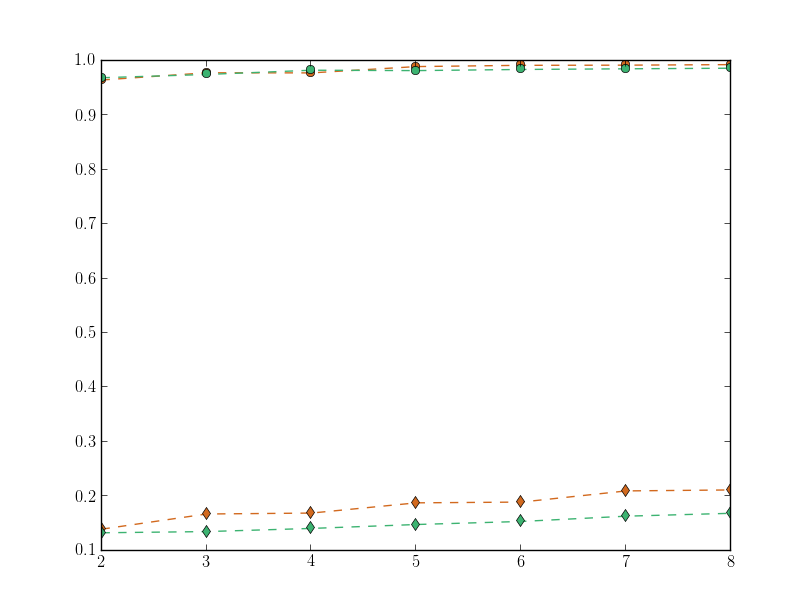
\includegraphics[width=0.50\textwidth, trim=15mm 10mm 9mm 0mm ,clip]{./img/clusteval1.png}&\begin{turn}{90}\scriptsize\hspace{1.5cm} score CCM \end{turn}&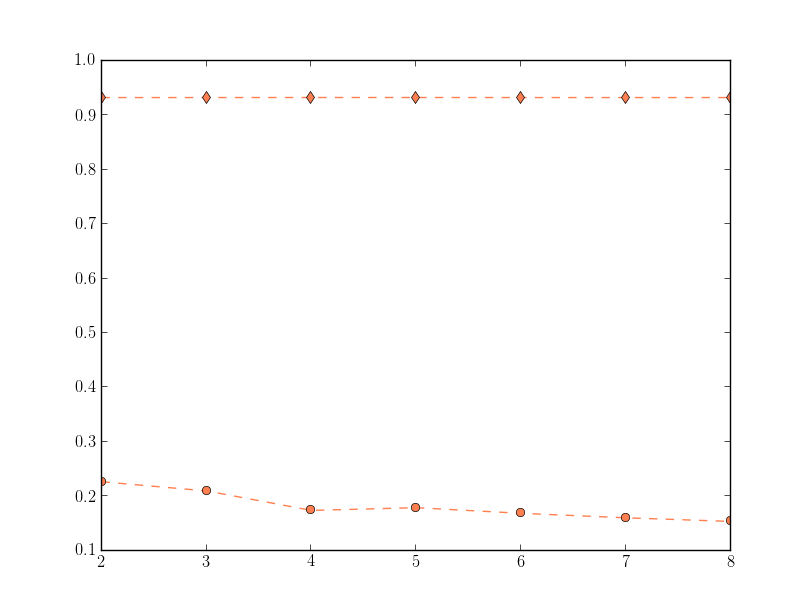
\includegraphics[width=0.50\textwidth, trim=15mm 10mm 9mm 0mm ,clip]{./img/clusteval2.png} \\
	&\scriptsize (A) Granularité&&\scriptsize (B) Granularité\\
	\end{tabular}
	\begin{tabular}{ccc}
	\begin{turn}{90}\scriptsize\color{blue}Nombre de clusters avec plus d'une protéines \end{turn}&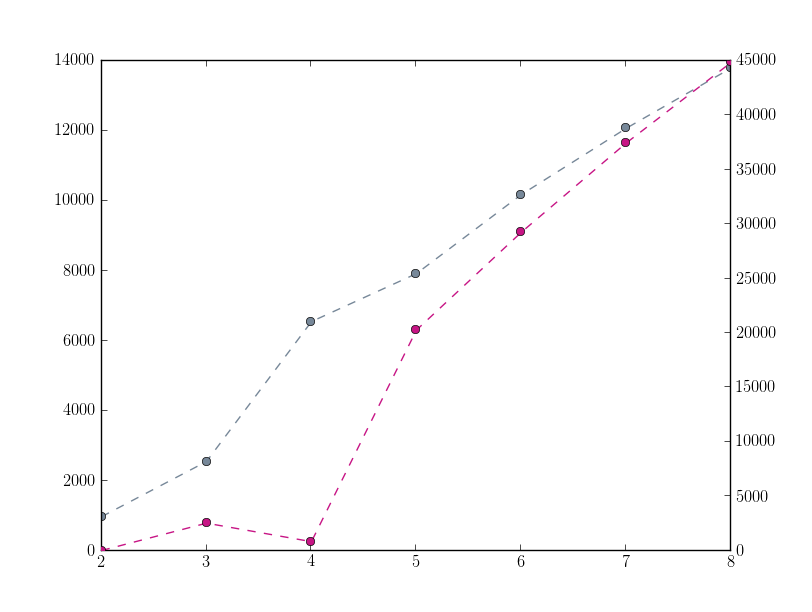
\includegraphics[width=0.50\textwidth, trim=15mm 10mm 9mm 0mm ,clip]{./img/clusteval3.png}&\begin{turn}{90}\scriptsize \color{magenta}\hspace{0.3cm}Nombre de clusters avec une protéine \end{turn}\\
	&\scriptsize (C) Granularité\\
	\end{tabular}
	\end{center}
	\caption[Influence de la granularité sur le clustering]{Influence de la granularité ($gr$) sur le clustering des protéines homologues des STIG. A: valeurs de BHI (orange), BHIw (vert). B: CCM (orange). C: Nombre de clusters de taille $>1$ (gris) et de taille $=1$ (rose). Losanges : résultats pour les clusterings engendrés aléatoirement.}\label{figclusteval}
	\end{figure}
    
Une augmentation de $gr$ semble accroître la performance de l'algorithme. Cependant, un $gr$ trop important ($gr\geq 3$) amplifie drastiquement le nombre total de clusters ainsi que le nombre de clusters ne contenant qu'une seule protéine. Une inflation trop importante semble ainsi avoir pour effet d'empêcher la détection de l'homologie entre protéines ou groupes de protéines, si elle est trop faible. Majorer $gr$ a donc pour effet de faire perdre de l'information entre protéines et entre réplicons, tout en renforçant la pertinence biologique des clusters (dans l'objectif d'avoir des clusters de protéines homologues au niveau fonctionnel). En imaginant des cas extrêmes, nous pouvons faire l'hypothèse qu'un $gr$ très important ne conservera l'homologie qu'entre des protéines très proches, appartenant vraisemblablement à des individus de la même espèce, et donc n'apportera pas d'information pertinente quant à la comparaison des différents réplicons. À l'inverse, un $gr$ trop faible aura pour tendance: i) de créer de fausses homologies entre certaines protéines et de produire des liens erronés entre réplicons, et ii) de créer des clusters de protéines non pertinents d'un point de vue biologique. \textbf{Un \textit{gr} de 4 apparaît ainsi être une valeur de travail pertinente}, pour laquelle les valeurs de CCM et BHIw sont améliorées (Figure \ref{figclusteval}).
\\
Un nombre raisonnable de clusters est produit tout en étant assez restrictif pour espérer séparer les groupes de protéines issues de familles multigéniques (Figure \ref{figclustersize}). La distribution en tailles $k$ des clusters (Figure \ref{figclustersize}) ne semble pas suivre de lois de probabilité classique.

\begin{figure}[H]
	\begin{center}
     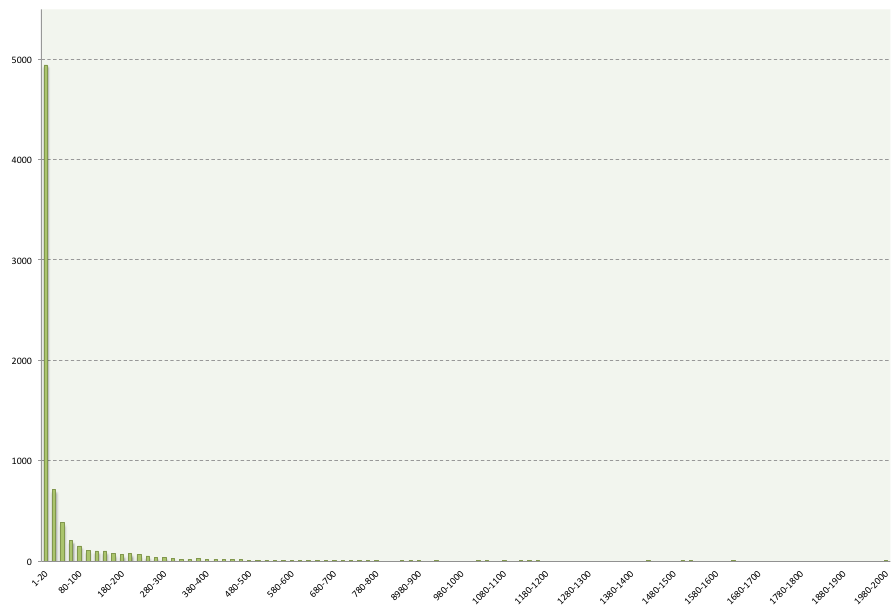
\includegraphics[width=0.8\textwidth]{./img/cluster_size.png}
    	\caption[Distribution de la taille des clusters de protéines pour $gr$ = 4]{Distribution de la taille des clusters de protéines pour un $gr$ de 4. \\ Abscisse : nombre de protéines par cluster. Ordonnée : nombre d'occurrence.}\label{figclustersize}
	\end{center}
\end{figure}
 
Malgré une très grande majorité de clusters homogènes obtenus pour un $Cl$ avec un $gr$ de 4 (Figure \ref{figannotdistib}), un faible pourcentage de clusters sont non-homogènes et regroupent des protéines ayant des annotations de fonctions proches (Table \ref{tabcausehetero}). Ce “bruit” semble être principalement lié à des familles multigéniques.
 \\

\begin{table}[H]
	\begin{center}
	\caption[Principales annotations multiples identifiées parmi les clusters]{Principales annotations multiples  identifiées parmi les clusters de protéines des STIG et pourcentage de ces annotations sur l'ensemble des clusters hétérogènes.}\label{tabcausehetero}
	\begin{tabular}{cc}
	\textbf{Annotations multiples} & \% \\
	\hline
	Ambiguïté XerC/XerD/Autres Xer & 38 \\
	Chromosomiques \textit{vs.} plasmidiques ParA & 11 \\
     Chromosomiques \textit{vs.} plasmidiques ParB & 6 \\
	Protéines DnaAB ambiguës & 5 \\
	Protéines Fts ambigües & 5 \\
     \end{tabular}
 \\ 
    
     \end{center}
\end{table}
     
\begin{figure}
      \begin{minipage}{0.5\textwidth}
      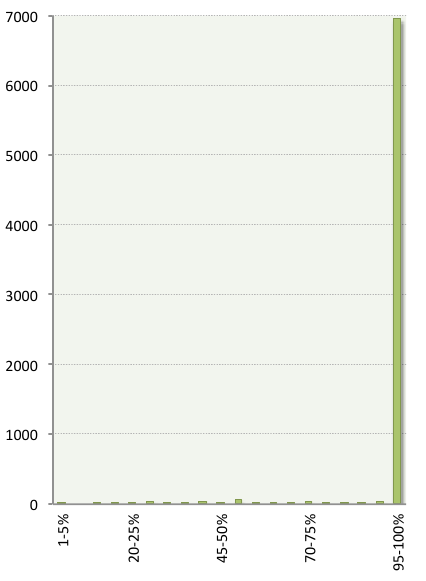
\includegraphics[width=\textwidth]{./img/protein_annot_distibA.png}
      \subcaption{}\label{figannotdistibA}
      \end{minipage}
      \begin{minipage}{0.5\textwidth}
      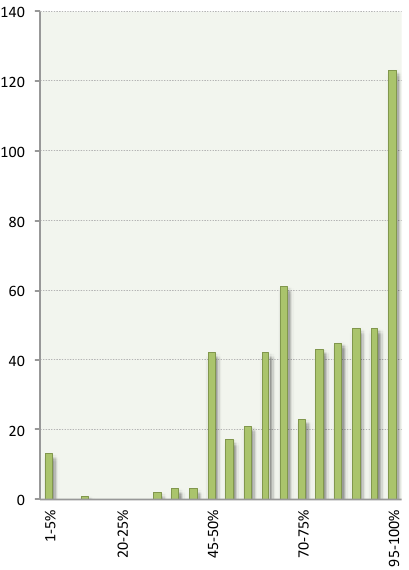
\includegraphics[width=\textwidth]{./img/protein_annot_distibB.png}            		\subcaption{}\label{figannotdistibB}
      \end{minipage}
      \caption[Pourcentage de l'annotation la plus fréquente par cluster]{Pourcentage de l'annotation la plus fréquente par cluster, parmi l'ensemble des clusters (\ref{figannotdistibA}) et parmi les clusters ayant des annotations multiples (\ref{figannotdistibB}). Les pourcentages sont calculés d'après l'éq. \ref{eqpourc}}\label{figannotdistib}.
\end{figure}    

\subsection{“Nettoyage” des clusters protéiques}\label{parcleaning}
	En raison de la présence de protéines avec des domaines fonctionnels multiples, un seuil de $10^{-5}$ pour l'analyse \textit{blastp} n'est pas suffisamment stringent pour garantir que la relation \ref{eqannot} est vérifiée dans tous les cas. Deux protéines partageant un même domaine fonctionnel peuvent être identifiées comme des homologues par une analyse de type \textit{blastp} bien que ne dérivant pas forcément d'une même protéine ancestrale \citep{Song2007}. Même si la question ici n'est pas de savoir si deux protéines ont une origine commune mais plutôt la même fonction, le problème reste identique: deux protéines peuvent posséder un domaine similaire (typiquement de type “transporteur ATP \textit{binding cassette}”, identifiant Pfam: ABC\_tran, par exemple) en addition d'un autre domaine, et cependant avoir des fonctions totalement différentes. Concrètement, on retrouve ce problème dans $P_{homo}$ avec, par exemple, l'obtention d'un cluster de protéines possèdant majoritairement un unique domaine de type “Sigma 54 modulation protein” (identifiant Pfam: Ribosomal\_S30AE). Ces protéines sont toutes liées à une protéine annotées XerC de \textit{Porphyromonas} (GI:332299940) qui comporte en plus d'un domaine de type intégrase, un domaine de type \textit{ABC\_tran}. Les protéines de ce cluster n'ont donc vraisemblablement pas le rôle d'intégrase et leur annotation XerC n'est donc pas pertinente.



\subsubsection{Procédure de nettoyage}
     Pour un cluster $C$, on définit son annotation $Ann(C)$ par:
	\begin{equation}
		Ann(C)=Ann(p) \iff N_{Ann(p)}^{C} = max\{N_{Ann(p_{i})}^{C}|\; p_{i} \in C \}
      \end{equation}
où $N_{Ann(p_{i})}^{C}$ désigne le nombre de fois que $Ann(p_{i})$ est trouvé pour les protéines de $C$.
Soit une protéine $p \in P$ avec $P=P_{ref} \cup P_{homo}$ et $D_{\{p\}}$ son ensemble de domaines fonctionnels. Le vecteur des domaines de $p$,  $v^{D_{P}}_{p}$, est alors introduit et est défini par: 
      \begin{equation}
		v^{D_{P}}_{p}=(N_{d_{1}}^{D_{\{p\}}},...,N_{d_{|D_{P}|}}^{D_{\{p\}}}),\;  d \in D_{P}
      \end{equation}
où $N_{d_{i}}^{D_{\{p\}}}$ est le nombre d'occurrences de $d_{i}$ dans $D_{\{p\}}$. Pour un cluster de protéines $C$, on peut définir son vecteur de domaines $v_{C}^{D_{P}}$ par:
      \begin{equation}
      	v_{C}^{D_{P}}=(\bar{N}_{d_{1}}^{C},...,\bar{N}_{d_{|D_{P}|}}^{C})
      \end{equation}
où $\bar{N}_{d_{i}}^{C}$ est défini par:
	\begin{equation}
       	\bar{N}_{d_{i}}^{C}=\frac{1}{|C|}\sum_{p \in C}N_{d_{i}}^{D_{\{p\}}}
	\end{equation}
Soit le clustering $Cl_{ref}$ formé des différentes groupes d'orthologues KEGG et familles ACLAME tel que $Cl_{ref}= Cl_{KEGG} \cup Cl_{ACLAME}$. Pour un clustering $Cl$ et pour tout $C_{i},C_{k} \in Cl$, on considère alors la distance:
      \begin{equation}\label{cleaningcosine}
      	d_{eval}(C_{i},C_{k})=d_{cosine}(v_{C_{i}}^{D_{P}},v_{C_{j}}^{D_{P}}) \textrm{ avec } \; C_{j} \in Cl_{ref} \textrm{ et } Ann(C_{k})=Ann(C_{j}) 
	\end{equation}       
avec $d_{cosine}$, la distance \textit{cosine}. Cette distance a une valeur unique pour chaque $C_{i}$ car il n'existe qu'un seul $C_{j} \in Cl_{ref}$ tel que $ Ann(C_{k})=Ann(C_{j})$. Soient un cluster $C_{i} \in Cl$ et un cluster aléatoire $C_{r}$ tels que $|C_{i}|=|C_{r}|$. Soit $X_{evalC_{i}}$, la variable aléatoire de $d_{eval}({C_{r},C_{i}})$ prenant ses valeurs dans $[0,+\infty[$. \textbf{On considère alors que $C_{i}$ est un cluster de $Cl$ valide si et seulement si:}
      \begin{equation}\label{eqseuil}
      	\begin{dcases}
      		d_{eval}(C_{r},C_{i})\leqslant x_{seuil_{i}}\\
      		P(x_{seuil_{i}} \leqslant X_{evalC_{i}})=0.90
      	\end{dcases}
      \end{equation}



\subsubsection{Estimation de $x_{seuil_{i}}$}
	Pour un cluster $C_{i} \in Cl$ donné, $n$ tirages avec remise de clusters aléatoires $C_{r_{i}}$ sont effectués avec $|C_{i}|=|C_{r_{i}}|$ en utilisant les estimations de $X_{d}$ et $X_{t}$ (relations \ref{Xd} et \ref{Xt}). Soient $Cl_{r_{i}}$ l'ensemble de ces clusters, $O_{Cr_{i}}=\{d_{eval}(C_{r_{i,1}},C_{i}),...,d_{eval}(C_{r_{i,n}},C_{i})\}$ l'ensemble des scores obtenus, et $Q_{O_{Cr_{i}}}^{10}$ ses déciles. On estime alors que:
     \begin{equation}
     x_{seuil_{i}}=x_{2/10}
	\end{equation}
	où  $x_{2/10}$ correspond à la première valeur du deuxième décile de $Q_{O_{Cr_{i}}}^{10}$.  



\subsubsection{Résultats et discussion}\label{parcleaningres}
	Cette procédure de cleaning consiste à évaluer si, pour un cluster de protéines $C$, les distributions en domaines fonctionnels de ses protéines se rapprochent de celles observées pour la famille de référence ayant la même annotation que $C$ ($Ann(C)=Ann(C_{ref})| \: C_{ref} \in Cl_{ref}$). On évalue avec l'éq.  \ref{cleaningcosine} la distance séparant les deux clusters. Les deux clusters ont des protéines ayant des domaines similaires si la distance observée est inférieure à 90\% des distances observées avec des clusters engendrés aléatoirement (éq. \ref{eqseuil}). \\
Le choix de la méthode de “cleaning”, ses performances, ainsi que de possibles méthodes alternatives sont discutés plus loin. Cependant, un des biais à souligner est celui lié à $D_{P_{homo}}$, qui intervient dans l'estimation de $X_{t}$ (éq. \ref{Xt}). À cause du jeu de protéines utilisé, certains domaines (tels que les domaines Pfam ABC\_tran ou Phage\_integrase) sont sur-représentés en comparaison à des domaines mineurs.  Ainsi, des clusters aléatoires formés avec des protéines comportant ces domaines seront plus probables et la méthode d'évaluation pour, par exemple, un petit cluster de recombinases sera plus restrictive. De plus, des protéines fausses positives $P_{FP}$ identifiées comme homologues à une protéine de référence multidomaines $p_{ref}$ peuvent avoir une partie de leurs domaines en commun avec $p_{ref}$ \citep{Song2007}, la procédure de cleaning ne prenant pas en compte ce biais dans la génération de clusters aléatoires. Enfin, un seuil de 10\% étant assez large, il en résulte que la procédure de cleaning est finalement peu restrictive et n'élimine que les clusters comportant des protéines présentant des distributions de domaines très biaisées par rapport à leurs familles de références $C_{ref}$ (Figure \ref{figannotclust}).\\ 
	En utilisant un $gr$ de 4, \textbf{917} clusters renfermant un total de \textbf{91.127} protéines, dont une large part est annotée “FtsE”, ont été identifiés comme n'étant pas valides (Figure \ref{figannotclust}A). Ces protéines sont vraisemblablement des membres de la superfamille des transporteurs ABC. Une partie importante des clusters valides est aussi annotée FtsE (Figure \ref{figannotclust}B). Ces protéines possèdent généralement un unique domaine ABC\_trans similairement aux “vraies” protéines FtsE. Il est alors probable que seules certaines d'entre elles ont une réelle fonction de type FtsE. On peut donc conclure que la seule utilisation de la distribution en domaines protéiques n'est pas toujours suffisamment discriminante pour l'identification des homologues fonctionnels. En considérant les seuils BLAST appliqués, on peut cependant supposer que ces protéines sont assez proches au niveau de leurs séquences et de leurs fonctions pour être tout de même maintenues dans notre jeu de données. 
	
\begin{figure}[H]
\begin{center}
\begin{subfigure}{0.7\textwidth}
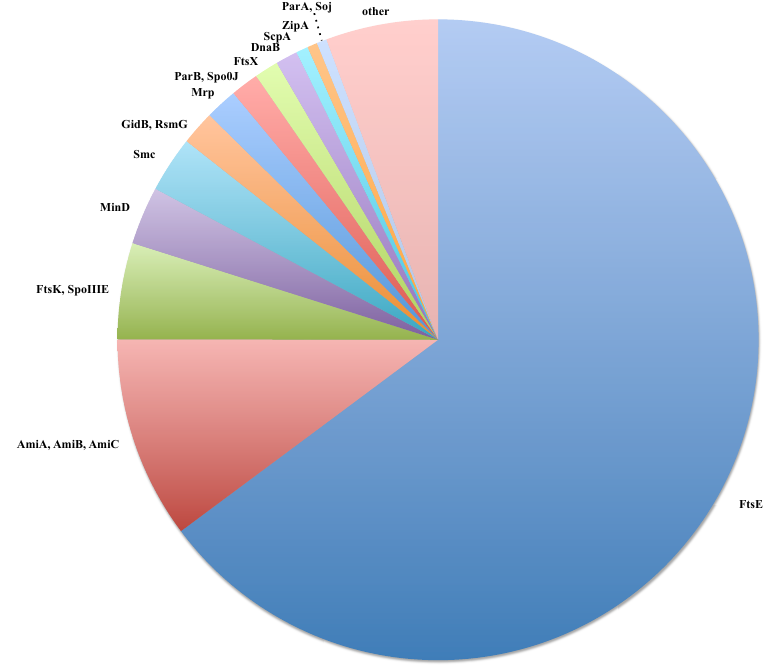
\includegraphics[width=\textwidth]{./img/cluster_noise.png}
\caption{Annotations des 917 clusters considérés comme \textit{incorrects}}
\end{subfigure}
\\
\vspace*{1cm}
\hspace{1cm}
\begin{subfigure}{0.8\textwidth}
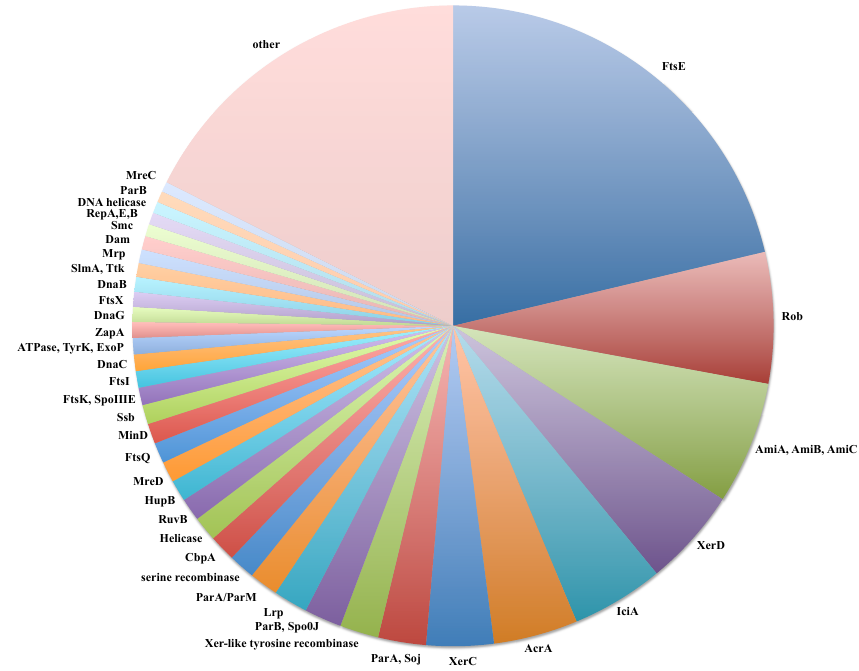
\includegraphics[width=\textwidth]{./img/cluster_annotate.png}
\caption{Annotations des 6465 clusters pertinents}
\end{subfigure}
\caption[Annotation des clusters de protéines]{Annotations des clusters de protéines. \\ Les clusters sont annotés selon l'annotation majoritaire des protéines qu'ils renferment (éq. \ref{eqannot}).}\label{figannotclust}
\end{center}
\end{figure}


\subsubsection{Alternatives à la procédure de cleaning} 
	D'un point de vue méthodologique, la procédure de cleaning utilisée est similaire à une procédure de classification supervisée, effectuée pour chaque cluster de protéines obtenu $C$ avec comme training set $E_{training}=\{E_{True},E_{False}\}$. D'une part, l'ensemble $C_{ref}$ des protéines a la même annotation que $C$ ($E_{True}$) et, d'autre part, des clusters de protéines engendrés aléatoirement $C_{r}$ selon la taille de $C$ correspondent à la distribution du type et du nombre de domaines de l'ensemble des protéines récupérées par l'analyse par \textit{blastp} ($E_{False}$). Différentes alternatives au calcul de la distance de l'éq. \ref{eqseuil} peuvent alors être envisagées:
\begin{description}
	\item[$\bullet$] Utiliser des algorithmes de classification supervisée classiques avec $E_{training}=\{C_{ref},C_{r}\}$. Les protéines, en fonction de leurs domaines, sont alors classées comme étant similaires à $C_{ref}$ ou à $C_{r}$ et, en fonction du nombre de protéines identifiées positives, $C$ est accepté ou refusé. Un des problèmes sous-jacents est de choisir les éventuels paramètres des algorithmes.
	\item[$\bullet$] Trier directement les protéines (et non les clusters) \underline{avant} d'effectuer la procédure de clustering par TRIBE-MCL. Un des inconvénients de cette approche est la possibilité d'éliminer des protéines $TP$ regroupées dans des clusters $TP$ grâce à leur homologie de séquence et étant de vrais positifs bien que n'ayant pas de domaines fonctionnels identifiés. Cela est toutefois peu probable, /\textit{hmmscan} étant beacoup plus sensible que /\textit{blastp}.
	\item[$\bullet$] Modifier $E_{training}$ en incluant, par exemple, un ensemble plus large de protéines témoins $TN$ dans $E_{False}$. Afin de compenser les biais introduits par des clusters $FP$ identifiés par l'analyse à cause de la présence d'un domaine commun avec certaines protéines $TP$,  $E_{False}$ pourrait être constitué de clusters de protéines aléatoires ayant la même annotation que les protéines de $E_{True}$. Il est cependant possible que cette procédure rende l'étape de cleaning beaucoup trop discriminative, en particulier pour les petits clusters. Il aurait été également intéressant de tester $C$ contre l'ensemble des $E_{True}$, et pas seulement contre l'ensemble présentant la même annotation que $C$, afin de  limiter les ambiguïtés pour les annotations proches comme XerC/XerD. 
	\item[$\bullet$] Inclure des données protéiques supplémentaires comme, par exemple, la taille et la synténie des domaines ou les données issues d'autres bases de données (TIGRFAM...).
	\item[$\bullet$] Utiliser une méthode tirée de la littérature pour la discrimination fonctionnelle des protéines par leurs domaines. Song \textit{et. al} \citep{song2008sequence} proposent une méthode similaire reposant sur une classification par régression logistique et des pondérations différentes des domaines et des séquences. Cependant, des problèmes similaires dans la classification de protéines ayant des domaines fréquents (exemple pKinase) sont mis en avant. Enfin, différentes alternatives à MCL peuvent être prometteuses dans l'identification d'homologues \citep{Terrapon2014}.
\end{description}

Trouver la procédure optimisant le nombre de protéine $TP$ présentes, homologues aux protéines de $P_{homo}$, et limitant le nombre de protéines $FP$ demande des études additionnelles qui n'ont pas été la priorité de cette étude. La difficulté, ici, est que les protéines de $P_{homo}$ appartiennent à différentes familles et présentent différents types d'homologies (Figure \ref{figtyrrec}). Ainsi, un cluster peut être constitué de l'aggrégation de différents sous-ensembles de protéines homologues et, inversement, différents clusters peuvent appartenir à un même niveau d'homologie. La structuration des clusters est de plus fortement influencée par le choix des paramètres, ici, $gr$ pour TRIBE-MCL, et dépend aussi des familles de protéines considérées.

\begin{figure}[H]
\Tree[.{tyrosine-recombinase} [ .Xer XerC XerD XerH ] [ .{tyrosine-intégrase} {phage-intégrase} {plasmide-intégrase} ] ]
\caption{Différents niveaux d'homologie chez les tyrosine-recombinases}\label{figtyrrec}
\end{figure}
